\documentclass[twocolumn,preprintnumbers,amsmath,amssymb,aps,prl]{revtex4}
\usepackage{graphicx,graphics}
\usepackage{float}
\usepackage{lipsum, babel}
\usepackage{dcolumn}
\usepackage{bm}
\usepackage{psfrag} 
\newcommand{\ket}[1]{|#1\rangle}        
\newcommand{\bra}[1]{\langle#1|}        
\newcommand{\braket}[2]{\langle#1|      #2\rangle}
\newcommand{\psfg}[1]{\psfrag{#1}{\S    mall{$#1$}}}

\begin{document}

\begin{abstract}
\textbf{Resumen.}
Se analizó el comportamiento de la disociación de moléculas a diferentes valores energéticos, para esto en un principio se resolvió la ecuación diferencial de $\Psi$ por medio de la ecuación de Riccati, la cual fue resuelta a través del lenguaje de programación \textbf{C++} con los métodos numéricos de \textbf{RK2} y \textbf{RK4}. Luego, se pusieron a prueba diferentes hombros de potencial con J$>$10 y se buscaron niveles energéticos que se encontraran atravesando la barrera centrifuga del potencial y por encima de esta, para posteriormente analizar sus funciones probabilísticas y graficarlas por medio del programa \textbf{Gnuplot}. 

\end{abstract}

\title{Disociación de moléculas, la ecuación de Riccati y Runge-Kutta.}
\author{Loaiza Ospina, Sebastian (1923876); Sinsajoa Duque, Ivan Ricardo (1926247).}

\maketitle

\section{Introducción.}
El estudio de los niveles energéticos dentro de una molécula ha sido un tema de discusión dentro de la física con el pasar de los años, en un principio el tema se abordó por medio de análisis clásicos los cuales no correspondían correctamente los resultados encontrados experimentalmente, pero con la llegada de la física cuántica los modelos teóricos se empezaron a ajustar de forma mas acorde a los resultados experimentales, la única dificultad detrás de los modelos cuánticos eran sus sistemas complejos, los cuales suelen ser tratados de forma computacional debido a que su solución analítica representa mayor esfuerzo. La utilización de métodos numéricos como lo son RK2 y RK4 permiten una solución mucho más sencilla y rápida.

Otro problema viene presente en las ecuaciones presentadas por el modelo teórico, ya que estas trabajan solo a valores muy específicos de energía, por lo mismo algunas soluciones otorgadas por la función $\Psi$ no representan una función de probabilidades y por lo mismo no son información relevante para el problema  a tratar, por esto mismo parte del trabajo a la hora de analizar estas funciones es encontrar estos valores de energía para los cuales sea posible modelar la función de onda, los cuales están asociados a los valores propios . 

Los métodos numéricos desarrollados a través de la historia nos permiten realizar funciones tales como la integración por medio de aproximaciones numéricas cada vez mas complejas y precisas, para sistemas de ecuaciones diferenciales complejos —como lo son las ecuaciones diferenciales radiales— los métodos numéricos nos permiten encontrar soluciones aproximadas mucho mas sencillas que el clasico metodo analítico, el cual suele estar lleno de procedimientos largos y poco prácticos que pueden tomar gran parte de nuestro tiempo y suelen ser de dificil comprensión.

Por ello la evolución de análisis en sistemas más complejos ha provocado la llegada de métodos computacionales más elaborados y estrucutarados que han permitido comprender los fenómenos que se observan en entornos tan anti-intuitivos como es el mundo atómico, permitiendo así el avance científico y tecnológico de la sociedad.

\section{Metodología.}

Considerando entonces una molécula formada por dos átomos alcalinos la energía del sistema satisface la siguiente ecuación diferencial radial:

\begin{equation}\label{E1}
    E\Psi(R)=-\frac{\partial^2\Psi(R)}{\partial R^2}+\left(\frac{J(J+1)}{R^2}+V(R)\right)\Psi(R)
\end{equation}

Donde J es el momento rotacional y $V(R)$ el potencial que modela la interacción entre los nucleos, y el cual en este caso es el potencial de morse que viene descrito de la siguiente forma:

\begin{equation}
    V(R)=D_e\left(1-e^{-\alpha(R-R_e)}\right)^2
\end{equation}

Donde $D_e$ es la profundidad del pozo, $R_e$ es la ubicación del minímo del potencial y $\alpha$ es una variable que controla el ancho del potencial (mientras más pequeño sea $\alpha $, más grande es el pozo).

De manera que para resolver la ecuación diferencial radial (1) se utilizó la ecuación de riccati, la cual afirma que para transformar una ecuación diferencial radial de segundo orden de la forma:
\begin{equation}\notag
    \frac{d^2y}{dx^2}=f(x)y(x)
\end{equation}
En una ecuación de primer orden no lineal, se define:
\begin{equation}\notag
    g=\frac{y'(x)}{y(x)}
\end{equation}

De manera que la ecuación (1) se puedede escribir como

\begin{equation}\notag
    g'+g^2=f(x)
\end{equation}

Y de forma explícita

\begin{equation}\notag
    g=\frac{\Psi'(R)}{\Psi(R)}
\end{equation}

\begin{equation}\notag
    g'+g^2=\frac{J(J+1)}{R^2}+V(R)-E
\end{equation}

Es decir el sistema de ecuaciones diferenciales acoplado a resolver sería.

\begin{equation}\label{E2}
    \Psi'(R)=g(R)\Psi(R)
\end{equation}

\begin{equation}
    g'=\frac{J(J+1)}{R^2}+V(R)-E-g^2
\end{equation}
Para ello entonces se consideraron valores de $J>10$ y valores arbitrarios para las constantes $D_e, R_e$ y $\alpha$. Sin embargo los valores de energía se ajustaron dependiendo de estas constantes para que el sistema tuviera la solución probabilística correcta. Además se tuvo en cuenta que la función g diverge en R=0 ya que la función $\Psi(0)=0$ por lo que se solucionó la ecuación es en la parte externa del potencial, es decir en el caso en que los átomos no alcanzan a sobrepasar la barrera y por tanto no forman una molécula, sin embargo por simplicidad se solucionó para cuando se genera molécula y despues se invirtió la gráfica, por ello se tomó la condición de función de onda $\Psi(R=Re)=1$ y una condición de $g(Re)$ que cumpliera con la relación (3).
A continuación, se muestra una tabla con los valores de constantes tomados para la solución

\begin{table}[h!]
    \centering
    \begin{tabular}{|c|c|}\hline
    Parámetro & Valor \\\hline
    $D_e$ & 8.0 \\\hline
    $R_e$ & 5.0 \\\hline
    $\alpha$& 3.0 \\\hline
    $J$ & 11 \\\hline
    $\Psi(Re)$ & 1 \\\hline
    $g(Re)$ & 0 \\\hline
    \end{tabular}
    \caption{Valores de constantes tomadas para el potencial de morse y condiciones iniciales para la solución de la ecuación diferencial.}
    \label{tabla1}
\end{table}

Por ultimo para resolver el sistema de ecuaciones (3) y (4) se hizo uso de los métodos numéricos RK2 y RK4 que fueron programados en C++. Las itineraciones fueron las siguientes 

\textbf{RK2}
\begin{eqnarray}\notag
y_{i+1}=y_i+(k_1+k_2)/2 \\\notag
x_{i+1}=x_i+(l_1+l_2)/2
\end{eqnarray}
En el cual sea $h=\frac{tf-t0}{n}$ entonces 
\begin{eqnarray}\notag
k_1&=&hf(t_i,x_i,y_i) \\\notag
k_2&=&hf(t_i+h,x_i+l_1,y_i+k_1) \\\notag
                                \\\notag
l_1&=&hy_i                    \\\notag
l_2&=&h(y_i+k_1)              
\end{eqnarray}
\textbf{RK4}
\begin{eqnarray}\notag
y_{i+1}=y_i+(k_1+2k_2+2k_3+k_4)/6 \\\notag
x_{i+1}=x_i+(l_1+2l_2+2l_3+l_4)/6
\end{eqnarray}
En el cual sea $h=\frac{tf-t0}{n}$ entonces 
\begin{eqnarray}\notag
k_1&=&hf(t_i,x_i,y_i) \\\notag
k_2&=&hf(t_i+\frac{h}{2},x_i+\frac{l_1}{2},y_i+\frac{k_1}{2}) \\\notag
k_3&=&hf(t_i+\frac{h}{2},x_i+\frac{l_2}{2},y_i+\frac{k_2}{2})\\\notag
k_4&=&hf(t_i+h,x_i+l_3,y_i+k_3)\\\notag
                                \\\notag
l_1&=&hy_i                    \\\notag
l_2&=&h(y_i+\frac{k_1}{2}) \\\notag
l_3&=&h(y_i+\frac{k_2}{3}) \\\notag
l_4&=&h(y_i+k_3) 
\end{eqnarray}
\section{Datos Y Resultados.}
A la hora de analizar la función $\Psi$ lo primero que se debe considerar son los valores arbitrarios que se le otorgaran a sus constantes, en este caso como se puede observar en la tabla \ref{tabla1}, nuestras constantes contaban con magnitudes poco comunes en problemas de este ámbito. Sin embargo, esto no quiere decir que no existan valores energéticos para los cuales tenga sentido la solución de la función $\Psi$. Una vez mencionado esto el siguiente análisis que se debe realizar es el del hombro del potencial, en este caso se estudiaron hombros de potencial con $J>10$ que realmente presentaran información relevante al problema.

Una vez otorgados todos estos valores el potencial de morse tendría la siguiente forma:

\begin{figure}[h!]
    \centering
    \includegraphics[width=0.5\textwidth]{Potencial.png}
    \caption{Potencial de morse visto a escala completa y zoom en el hombro del potencial.}
    \label{fig1}
\end{figure}

Luego de encontrar el potencial de morse, se buscaron diferentes valores energeticos para solucionar la función $\Psi$, donde se encontró lo siguiente.

Para valores energéticos pequeños la función $\Psi$ se modelaba en forma de función exponencial.

\begin{figure}[h!]
    \centering
    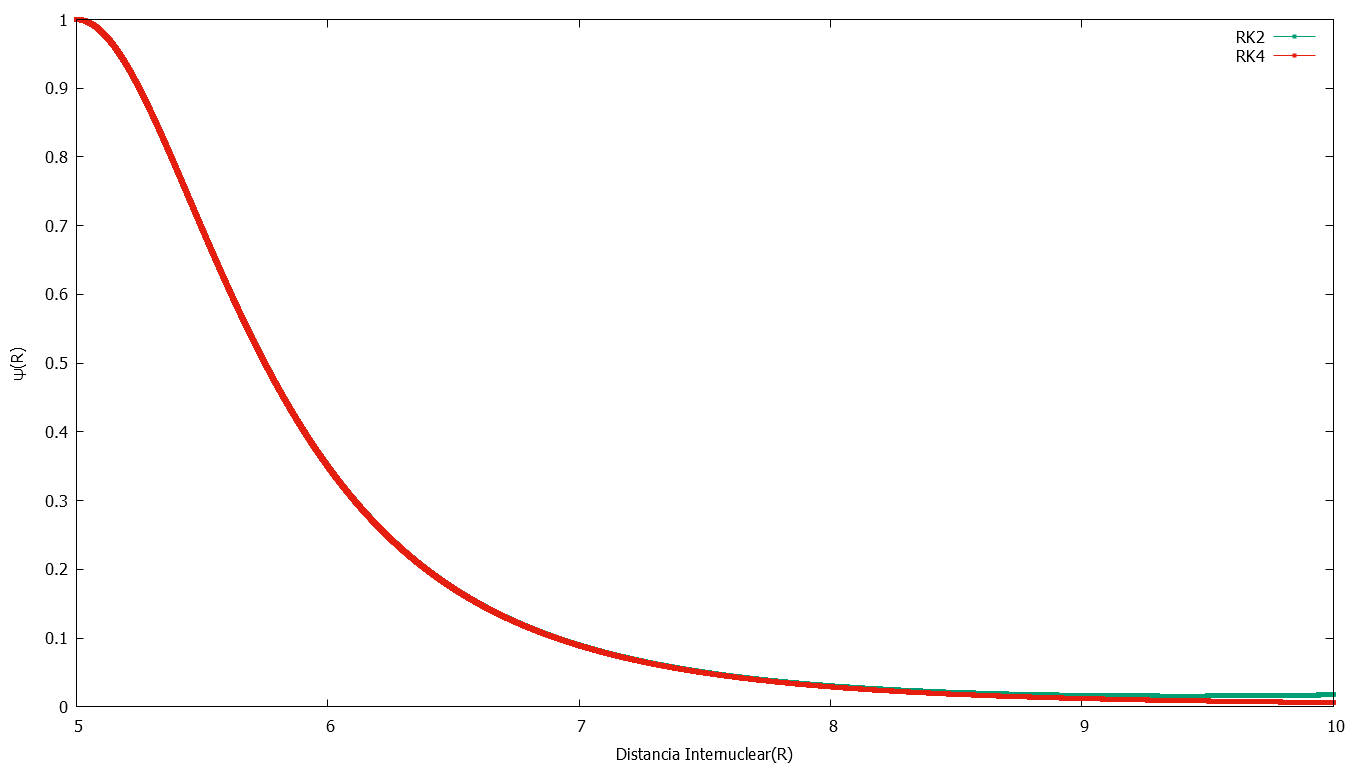
\includegraphics[width=0.45\textwidth]{E1.png}
    \caption{Grafica de la función $\Psi$ con $E<8.83167$.}
    \label{fig2}
\end{figure}
Para el valor $E=8.83167$ la función $\Psi$ se modela en forma de función probabilística.

\begin{figure}[h!]
    \centering
    \includegraphics[width=0.45\textwidth]{E2.png}
    \caption{Gráfica de la función $\Psi$ con $E=8.83167$. Para este valor en específico $\Psi$ si representa una función de probabilidades.}
    \label{fig3}
\end{figure}
Para valores energéticos elevados la función $\Psi$ se modelaba en forma de función senosoidal.
\begin{figure}[h!]
    \centering
    \includegraphics[width=0.45\textwidth]{E3.png}
    \caption{Grafica de la función $\Psi$ con un valor enérgetico $E>8.83167$.}
    \label{fig4}
\end{figure}

Finalmente para observar el funcionamiento de todo el modelo, se grafico el potencial de morse y la funcion probabilistica en una misma escala de (R) con el fin de ver como el potencial de morse influye en la probabilidad de formacion de una molecula respecto al radio. Se utilizaron las mismas constantes

\begin{figure}[h!]
    \centering
    \includegraphics[width=0.45\textwidth]{g1.png}
    \caption{Potencial de morse junto a la barrera centrifuga en los ejes XY y la Funcion probabilistica en los ejes X2Y2.}
    \label{fig5}
\end{figure}

\section{Conclusiones.}
La función de probabilidades $\Psi$(R) solo muestra soluciones válidas para valores específicos de E, los cuales están dados por las diferentes constantes de la función y el valor J, que determina el hombro del potencial.

La solución de la función $\Psi$(R) modela la probabilidad de que exista o no molécula para cada valor de R, en casos para los cuales queremos calcular la probabilidad de que no exista molécula,por ello es natural ver como la función de probabilidades empieza en 0 y termina en 1.

Los métodos numéricos de Runge-Kutta son una aproximación valida a la solución del problema, y en este caso debido a que se trabajó en una caja de solución para valores de R pequeños la diferencia entre RK2 y RK4 fue prácticamente imperceptible debido a esto solo se graficó RK4. Sin embargo si se trabajara con valores de R más grandes se vería la diferencía. Esto no fue poisble debido a que para valores de R más grandes la ecuación de Riccati se volvía cada vez más inexacta y no permitía un análisis apropiado del sistema y por ende no era posible comparar RK2 y RK4.

Para valores energéticos muy pequeños la función $\Psi$(R) presenta soluciones en forma de función exponencial, mientras que, para valores energéticos muy grandes, las soluciones de la función $\Psi$(R) son ondas que oscilan hasta el infinito. Sin embargo, ninguna de estas dos soluciones tiene significado relevante para el problema a estudiar, por lo que ambas se consideran errores de cálculo.

A pesar de haberse encontrado el valor exacto de $E$ para la cual $\Psi$ si representa una función de probabilidades. Realmente faltaría el paso de normalización para que esta pueda llevarse completamente a un análisis real. Por tanto en este caso $\Psi$ solo representa el paso anterior a su verdadera función de probabilidades.

\textbf{Link del video:}
\vspace{0.1}
https://drive.google.com/file/d/1ObIY4
fTtpqkNqTXyq_jlTrXylx7kNt50/view?usp=sharing

\begin{thebibliography}{3}
 \bibitem{ref1} M. Berrondo, J. Recamier. Resonances and antibound states in a Morse potential. International Journal of Quantum Chemistry, Vol 62, 239-244 (1998). 12ª edición, 2009. Páginas 794-822.
\bibitem{ref2} Fidiani, E. (2016). Modeling of diatomic molecule using the Morse potential and the Verlet algorithm..
\bibitem{ref3} Znojil, M. (2016). Morse potential, symmetric Morse potential and bracketed bound-state energies. Modern Physics Letters A, 31(14)

\end{thebibliography}


\end{document}
